\documentclass[10pt]{article}
% De-anonymized preprint mode (for arXiv): shows author names, no "under review" header.
% For an anonymous TMLR submission instead, use \usepackage{tmlr}.
% For the published camera-ready, use \usepackage[accepted]{tmlr}.
% Requires the TMLR style file: https://github.com/JmlrOrg/tmlr-style-file
\usepackage[preprint]{tmlr}
\usepackage{amsmath,amssymb}
\usepackage{booktabs}
\usepackage{graphicx}
\usepackage{url}
\usepackage[hidelinks]{hyperref}

\title{An Optimal Repetition Spacing for In-Weight Fact Retention}

\author{\name Aniket Mittal \email aniket\_mittal@berkeley.edu \\
      \addr University of California, Berkeley}

\begin{document}
\maketitle

\begin{abstract}
When a language model is fine-tuned to memorize a fact from repeated exposures, does it matter
whether those exposures are packed together or spread across training? We show that it matters a
great deal, and that the relationship is non-monotone. Holding the number of exposures and the
total amount of training fixed, and varying only the spacing between a fact's repeated exposures,
recall of the fact follows an inverted-U in the spacing: cramming the repetitions together and
spreading them maximally far apart both give poor retention, while an intermediate spacing is best.
On a 360M-parameter model the optimum recovers near-perfect recall (0.99) while the massed and
maximally spaced schedules reach only 0.22 and 0.31, a gap of about 0.7 that is stable across seeds.
The inverted-U replicates across four model families, and its magnitude tracks how hard the fact is
to memorize: the effect is large when memorization is difficult and shrinks toward the ceiling when
it is easy. The optimum also governs durable retention, not just end-of-training recall: after
continued training on unrelated text, well-spaced facts survive better than massed ones. The result
reconciles two lines of prior work, one reporting that spacing helps and one reporting that spacing
has little effect on memorization, as two views of a single non-monotone curve, and it gives a
concrete, tunable knob for anyone teaching facts to a model by repeated exposure.
\end{abstract}

\section{Introduction}

Teaching a model a specific fact, whether for editing, personalization, or continual learning,
usually means presenting that fact several times during training. A practitioner controls not only
how many times a fact appears but \emph{when}: the repeated exposures can be packed into a short
window or spread across the run. This spacing is a free parameter that is rarely examined.

We examine it directly. Fixing the number of exposures per fact and the total training budget, and
varying only the temporal spacing between a fact's repeats, we measure end-of-training recall over
a population of facts. Recall is a non-monotone function of spacing with an interior optimum:
retention is worst when repeats are massed together, improves as they are spread out, peaks at an
intermediate spacing, and then falls sharply when the repeats are spread maximally far apart.

This connects two strands of prior work that appear to disagree. One strand reports that spacing
or interleaving improves generalization in neural network training; another reports that larger
inter-repetition gaps reduce memorization. Our curve contains both: increasing spacing helps up to
the optimum and hurts past it. The apparent disagreement is a matter of which side of the optimum
each study sampled.

Our contributions are:
\begin{enumerate}
\item An inverted-U relationship between repetition spacing and in-weight fact retention, isolated
by a design that holds exposure count and total training fixed so that only spacing varies
(Section~\ref{sec:invertedU}, Figure~\ref{fig:invertedU}). The effect is large (about 0.7 in recall
between the optimum and the endpoints) and stable across seeds.
\item The optimum governs durable retention, not just end-of-training recall: after continued
training on unrelated text, well-spaced facts survive better (Section~\ref{sec:retention}).
\item The inverted-U replicates across four model families, with its magnitude tracking how hard the
fact is to memorize (Sections~\ref{sec:scaling}--\ref{sec:families}).
\end{enumerate}

\section{Related work}
\label{sec:related}

Our finding connects to a long line of behavioral research on the spacing effect, one of the most
reproducible results in the study of human memory. \citet{cepeda2006distributed} synthesized
several hundred experiments showing that distributing repetitions of study material over time
yields more durable retention than massing them together, and that the optimal interstudy interval
grows with the retention interval. \citet{cepeda2008spacing} sharpened this into a temporal
ridgeline: as the gap between repetitions increases, final-test performance first rises and then
falls, tracing an inverted-U whose peak shifts with test delay. Our result is a direct in-weight
analogue of that ridgeline. Holding exposure count and total training fixed and varying only the
temporal spacing of a fact's repetitions, we find best retention at an intermediate spacing, with
both massed and maximally spread schedules underperforming. The non-monotone shape that
\citet{cepeda2008spacing} describe for human learners appears here in the parameters of a
fine-tuned language model.

Within neural network training, prior work has largely studied repetition through its count rather
than its timing. \citet{carlini2022quantifying} show that extractable memorization grows
log-linearly with the number of times a sequence is duplicated, and \citet{lee2022deduplicating}
show that removing near-duplicate sequences reduces memorized emissions roughly tenfold while
preserving accuracy. \citet{allenzhu2024capacity} vary the number of exposures per fact and report
that knowledge storage falls from about two bits per parameter at a thousand exposures to about one
bit at a hundred. All three isolate how often a fact is seen; none manipulates when the repetitions
occur relative to one another. Our design fixes exposure count and isolates spacing, and it shows
that timing carries retention signal that frequency-only accounts miss.

The most direct point of comparison is \citet{tirumala2022memorization}, who periodically inject
held-out examples during training and measure a forgetting baseline. They report that the frequency
of repeated injection raises retention on the order of $10^{-2}$, whereas spaced repetition has
minimal effect, on the order of $10^{-3}$ and roughly independent of the spacing length, and they
read this as evidence that language models do not exhibit a human-like spacing benefit. Our results
diverge from that reading. Measuring semantic fact retention rather than verbatim memorization of
injected sequences, and sweeping spacing across its full range at fixed exposure count, we recover
a pronounced dependence on spacing with an interior optimum. The apparent null in
\citet{tirumala2022memorization} is consistent with sampling a region of the spacing axis where the
curve is flat, or with a memorization metric less sensitive to the retention differences spacing
produces. Framing the effect as an inverted-U rather than a monotone benefit reconciles the two
observations, since near the peak the retention gradient with respect to spacing is small.

A parallel literature on data ordering and scheduling situates the practical side of the result.
Work on curriculum learning arranges examples by difficulty or quality, and studies such as
\citet{beukers2024blocked} examine blocked versus interleaved schedules for learning multiple
schemas, but these address the order in which distinct items appear rather than the spacing of
repetitions of one item. \citet{prakriya2024lfr} come closest in spirit, revisiting forgotten data
regions at intervals in a manner explicitly motivated by spaced repetition, though they treat
spaced revisiting as an efficiency heuristic for pretraining loss rather than as a controlled
variable governing single-fact retention. Continual-learning research documents that continued
training erodes previously acquired knowledge \citep{luo2023empirical}, which explains why
maximally spread schedules can hurt in our setting as intervening updates overwrite an early
exposure. None of this work fixes exposure count and total compute to isolate spacing, and none
reports an interior optimum. Our contribution is to identify that optimum, show it holds across
model families, and connect it to the classical spacing ridgeline.

\section{Setup}
\label{sec:setup}

\paragraph{Facts.} We construct a pool of independent synthetic facts of the form ``The guardian of
$S$ is $O$,'' where each subject $S$ and object $O$ is an invented token, so the facts cannot be
recalled from pretraining. Each fact is presented $N$ times during training. Between and around the
fact exposures we insert a fixed stream of neutral filler text, so that the total training length
is the same regardless of spacing.

\paragraph{The spacing variable.} We control a gap fraction $g \in [0,1]$. For a given $g$, each
fact's $N$ exposures are spread evenly across a window covering a fraction $g$ of the training
stream: $g=0$ places all $N$ exposures back to back (massed), and $g=1$ spreads them across the
entire run (maximally spaced). Critically, the number of exposures $N$, the number of facts, the
filler count, the total number of optimizer steps, and the learning rate are identical across all
values of $g$. Only the positions of each fact's repeats change. Any difference in recall is
therefore attributable to spacing and not to how much a fact was seen or how long training ran.

\paragraph{Training and metric.} We fine-tune with LoRA~\citep{hu2022lora} and train on the ordered stream (we do not
shuffle, since the order is the manipulation). After training we measure recall as the fraction of
facts for which the model assigns the highest log-probability to the correct object among all
object candidates in the pool. This is a population statistic over the fact pool and does not
depend on brittle string matching.

\section{An inverted-U in repetition spacing}
\label{sec:invertedU}

Figure~\ref{fig:invertedU} shows recall as a function of the gap fraction $g$ on
SmolLM2-360M, averaged over three seeds. The curve is a clear inverted-U. Massed training ($g=0$)
gives recall $0.22 \pm 0.06$. Recall rises steadily with spacing, to $0.73$ at $g=0.2$, $0.92$ at
$g=0.5$, and a peak of $0.99$ around $g=0.65$ to $0.8$. It then collapses to $0.31 \pm 0.08$ at
maximal spacing ($g=1$). The interior optimum exceeds both endpoints by about $0.69$ in recall,
which is more than fifteen standard deviations given the across-seed spread. The error bars are
small at the peak (standard deviation $0.008$) and larger at the endpoints, but the ordering is
unambiguous in every seed.

\begin{figure}[h]
\centering
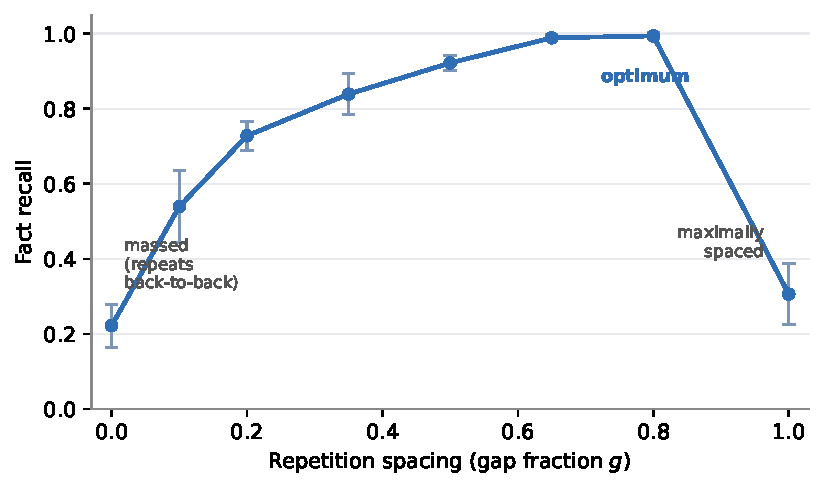
\includegraphics[width=0.72\linewidth]{fig_spacing_invertedU.pdf}
\caption{Fact recall as a function of repetition spacing $g$, holding exposure count and total
training fixed (SmolLM2-360M, three seeds, error bars one standard deviation). Both massed ($g=0$)
and maximally spaced ($g=1$) schedules retain poorly; an intermediate spacing is best.}
\label{fig:invertedU}
\end{figure}

Two features are worth noting. First, the rise from massed to the optimum is smooth, consistent
with spacing steadily improving consolidation. Second, the fall at maximal spacing is abrupt: when
a fact's few exposures are scattered across the whole run, the earliest exposures are effectively
overwritten by intervening training before the fact is consolidated. The optimum balances these,
spacing repeats far enough apart to benefit from spacing but close enough that the fact is
reinforced before it decays.

\section{The optimum governs durable retention, not just end-of-training recall}
\label{sec:retention}

End-of-training recall could in principle reflect how recently a fact was seen rather than how well
it was consolidated. To separate these, we continued training on filler text only, with no further
fact exposures, and re-measured recall. If spacing improved only recency, the advantage of the
optimal schedule would wash out under continued training; if it improved consolidation, the
advantage would persist. Figure~\ref{fig:retention} shows both curves.

\begin{figure}[h]
\centering
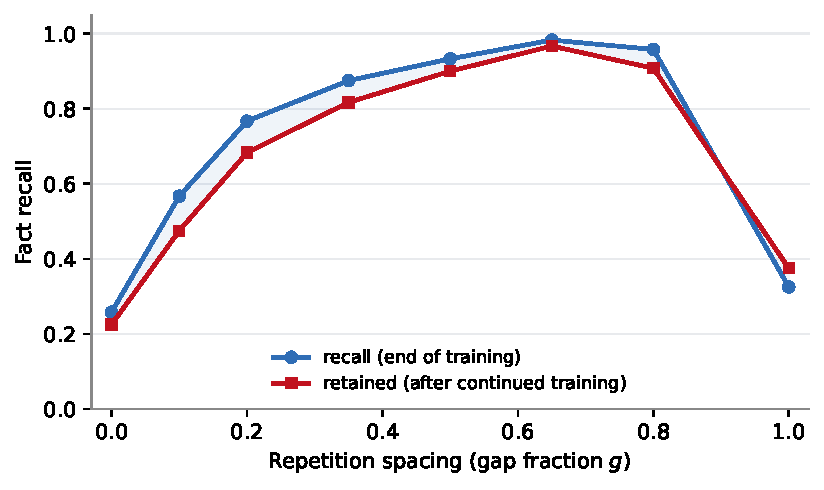
\includegraphics[width=0.70\linewidth]{fig_spacing_retention.pdf}
\caption{Recall at the end of training and after continued filler-only training (SmolLM2-360M, mean
over seeds). Retained recall is also an inverted-U with the same interior optimum, and the fraction
of recall that survives continued training rises with spacing.}
\label{fig:retention}
\end{figure}

Retained recall is itself an inverted-U with the optimum in the same place ($g=0.65$). Moreover, the
fraction of recall that survives continued training increases with spacing, from about 87\% for the
massed schedule to about 98\% at the optimum. Well-spaced facts are not only learned better, they
are more durable: they resist being overwritten by subsequent training. This supports the
consolidation account and rules out a pure-recency explanation.

\section{When spacing matters: the role of memorization difficulty}
\label{sec:scaling}

The size of the spacing effect depends on how hard the fact is to memorize, which in turn depends
on the learning rate. We swept the gap $g$ at several learning rates, controlling for the amount of
learning: because a larger learning rate memorizes a fact in fewer passes, we scaled the number of
training epochs inversely with the learning rate so that total learning pressure is comparable
across conditions. This control matters. Without it, a low learning rate simply fails to memorize
the facts at all, and its recall curve is flat and near the floor for every spacing, which would
spuriously suggest that the optimum has moved.

With learning pressure held comparable, the picture is consistent (Table~\ref{tab:difficulty}). In
conditions where the fact is hard to memorize, recall sits in a sensitive range and the inverted-U
is pronounced: the optimum exceeds the worst endpoint by about 0.7 in recall. In conditions where
the fact is easy to memorize, recall approaches the ceiling across most of the spacing range and the
curve flattens; for a low learning rate trained long enough to saturate, the optimum beats the worst
endpoint by only about 0.07, and the schedule barely matters. The location of the optimum does not
move systematically with learning rate once memorization is equalized; what changes is the amplitude
of the effect. Spacing is a lever that is strongest exactly where retention is otherwise most
fragile.

\begin{table}[h]
\centering
\begin{tabular}{llccccc}
\toprule
Model & Learning rate & Memorization & $g^\star$ & Massed & Max-spaced & Effect size \\
\midrule
SmolLM2-360M & $1\times10^{-4}$ & easy (saturated) & --- & 0.93 & 1.00 & 0.07 \\
SmolLM2-360M & $3\times10^{-4}$ & hard & 0.8 & 0.27 & 0.38 & 0.72 \\
Qwen2.5-1.5B & $3\times10^{-4}$ & hard & 0.8 & 0.21 & 0.53 & 0.78 \\
\bottomrule
\end{tabular}
\caption{The spacing effect scales with memorization difficulty, not with a shift in the optimum.
Learning pressure is equalized across learning rates by scaling epochs inversely with the learning
rate. Effect size is peak recall minus the worse of the two endpoints (massed, max-spaced), averaged
over three seeds. When memorization is easy, recall saturates and the effect nearly vanishes; when
it is hard, the inverted-U is large.}
\label{tab:difficulty}
\end{table}

We note that an earlier, uncontrolled version of this sweep appeared to show the optimum sliding to
smaller gaps at low learning rates. That apparent shift was an artifact of the low-learning-rate
conditions failing to memorize; once learning is equalized across rates, the shift disappears. We
report this because the controlled result is the correct one and the uncontrolled version is a
natural trap.

\section{Replication across model families}
\label{sec:families}

To test that the inverted-U is not specific to one architecture, we ran the same gap sweep, with
identical settings, on four model families: SmolLM2-360M, Qwen2.5-1.5B, Llama-3.2-1B, and
Gemma-2-2b (three seeds each). Figure~\ref{fig:families} shows the resulting curves.

\begin{figure}[h]
\centering
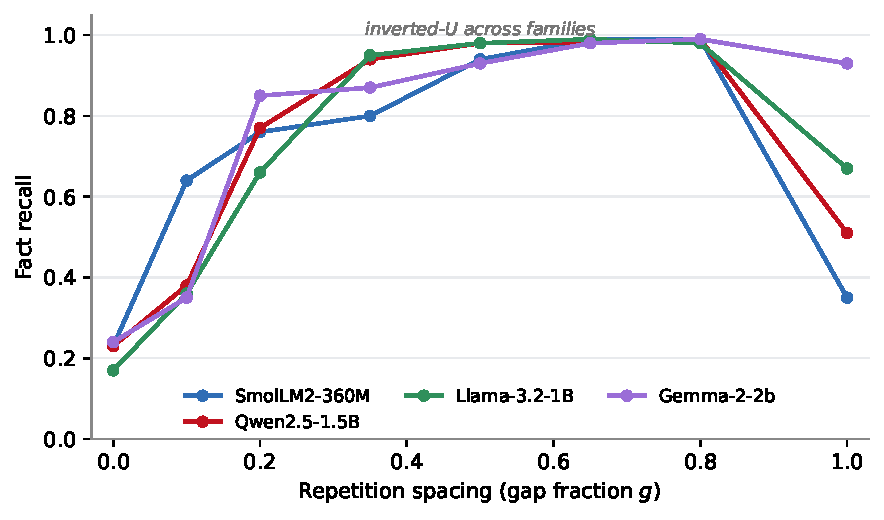
\includegraphics[width=0.74\linewidth]{fig_spacing_families.pdf}
\caption{Recall as a function of spacing $g$ across four model families (mean over seeds, base
learning rate). Three families show a pronounced inverted-U; Gemma-2-2b shows the same interior
peak but a muted decline at large spacing.}
\label{fig:families}
\end{figure}

The inverted-U replicates. SmolLM2-360M, Qwen2.5-1.5B, and Llama-3.2-1B all show the same shape:
low recall when massed (0.19 to 0.26), a peak of 0.99 at an interior gap ($g$ between 0.65
and 0.8), and a clear decline at maximal spacing (to 0.35, 0.53, and 0.68 respectively). The
optimum sits in the same region across these three families.

Gemma-2-2b is a partial exception that is informative rather than contradictory. It shows the same
interior peak (0.99 at $g=0.8$) and the same poor massed performance (0.24), but its recall at
maximal spacing stays high (0.93), so the inverted-U is muted at the upper end. Gemma-2-2b memorizes
these facts more readily than the other models, so even the less favorable schedules retain well and
the effect is compressed near the ceiling. This is consistent with the pattern in
Section~\ref{sec:scaling}: the spacing effect is largest when the fact is hard to memorize and
shrinks toward the ceiling when it is easy. The direction of the effect is preserved in all four
families; its magnitude depends on how difficult the fact is for the model to acquire.

\section{Discussion}
\label{sec:discussion}

\paragraph{Reconciling opposing prior claims.} The inverted-U resolves an apparent disagreement in
the literature. Human-memory research reports that spacing helps retention up to an optimum
\citep{cepeda2008spacing}, while a controlled study of language-model memorization reports that
spacing has essentially no effect \citep{tirumala2022memorization}. Our curve contains both
observations. Increasing spacing improves retention up to the optimum and degrades it past the
optimum, so a study that samples near the peak, or that varies spacing over a narrow range, will
see little dependence on spacing, while one that samples the full range will see a strong effect.
The reported null and the reported benefit are two views of the same non-monotone curve.

\paragraph{Why both ends are bad.} Two mechanisms bound the optimum. When repetitions are massed,
the fact is presented in a short window and the model has little opportunity to consolidate it
against interleaved material before training moves on, so it is under-reinforced. When repetitions
are maximally spread, the earliest exposures are separated from the latest by most of the training
run, and intervening updates overwrite them before the fact is reinforced, an effect consistent
with forgetting under continued training \citep{luo2023empirical}. The optimum spaces repetitions
far enough apart to benefit from interleaving but close enough that each exposure is reinforced
before it decays.

\paragraph{Practical guidance.} For anyone teaching a model a fact by repeated exposure, the
schedule is a free parameter worth setting deliberately. Neither cramming the repetitions together
nor scattering them across the whole run is a good default; an intermediate spacing recovers
substantially better retention at no additional data or compute. The effect is largest in the
regime where the fact is otherwise hard to memorize; when a fact is easy to memorize, recall
approaches ceiling regardless of spacing and the schedule matters less (Section~\ref{sec:scaling}).

\paragraph{Limitations.} Our study uses LoRA fine-tuning on synthetic facts with invented entities,
which isolates the manipulation but leaves open whether the same optimum governs natural facts that
interact with pretraining knowledge. The facts are single subject-relation-object triples; whether
the optimum shifts for longer or compositional knowledge is future work. Retention is measured
after a fixed amount of continued training; the dependence of the optimum on the length of that
continued training, analogous to the test-delay dependence in human studies
\citep{cepeda2008spacing}, is a natural next step.

\section*{Reproducibility}
Experiments run on a Modal and PEFT harness. Code and figures are released at
\url{https://github.com/aniket-mittal/spacing-fact-retention}. The script
\texttt{exp\_spacing\_law.py} reproduces the gap sweep, the multi-family replication, the retention
measurement, and the confound-controlled learning-rate sweep.

\begin{thebibliography}{99}

\bibitem[Allen-Zhu and Li(2024)]{allenzhu2024capacity}
Allen-Zhu, Z. and Li, Y. (2024).
\newblock Physics of Language Models: Part 3.3, Knowledge Capacity Scaling Laws.
\newblock \emph{ICLR 2025}. arXiv:2404.05405.

\bibitem[Beukers et al.(2024)]{beukers2024blocked}
Beukers, A. O., Collin, S. H. M., Kempner, R. P., Franklin, N. T., Gershman, S. J., and Norman, K. A. (2024).
\newblock Blocked training facilitates learning of multiple schemas.
\newblock \emph{Communications Psychology}, 2. DOI:10.1038/s44271-024-00079-4.

\bibitem[Carlini et al.(2022)]{carlini2022quantifying}
Carlini, N., Ippolito, D., Jagielski, M., Lee, K., Tram\`er, F., and Zhang, C. (2022).
\newblock Quantifying Memorization Across Neural Language Models.
\newblock \emph{ICLR 2023}. arXiv:2202.07646.

\bibitem[Cepeda et al.(2006)]{cepeda2006distributed}
Cepeda, N. J., Pashler, H., Vul, E., Wixted, J. T., and Rohrer, D. (2006).
\newblock Distributed practice in verbal recall tasks: A review and quantitative synthesis.
\newblock \emph{Psychological Bulletin}, 132(3):354--380.

\bibitem[Cepeda et al.(2008)]{cepeda2008spacing}
Cepeda, N. J., Vul, E., Rohrer, D., Wixted, J. T., and Pashler, H. (2008).
\newblock Spacing effects in learning: A temporal ridgeline of optimal retention.
\newblock \emph{Psychological Science}, 19(11):1095--1102.

\bibitem[Hu et al.(2022)]{hu2022lora}
Hu, E. J., Shen, Y., Wallis, P., Allen-Zhu, Z., Li, Y., Wang, S., Wang, L., and Chen, W. (2022).
\newblock LoRA: Low-Rank Adaptation of Large Language Models.
\newblock \emph{ICLR}. arXiv:2106.09685.

\bibitem[Lee et al.(2022)]{lee2022deduplicating}
Lee, K., Ippolito, D., Nystrom, A., Zhang, C., Eck, D., Callison-Burch, C., and Carlini, N. (2022).
\newblock Deduplicating Training Data Makes Language Models Better.
\newblock \emph{ACL 2022}. arXiv:2107.06499.

\bibitem[Luo et al.(2023)]{luo2023empirical}
Luo, Y., Yang, Z., Meng, F., Li, Y., Zhou, J., and Zhang, Y. (2023).
\newblock An Empirical Study of Catastrophic Forgetting in Large Language Models During Continual Fine-tuning.
\newblock arXiv:2308.08747.

\bibitem[Prakriya et al.(2024)]{prakriya2024lfr}
Prakriya, N., Yen, J.-N., and Hsieh, C.-J. (2024).
\newblock Accelerating Large Language Model Pretraining via LFR Pedagogy: Learn, Focus, and Review.
\newblock arXiv:2409.06131.

\bibitem[Tirumala et al.(2022)]{tirumala2022memorization}
Tirumala, K., Markosyan, A. H., Zettlemoyer, L., and Aghajanyan, A. (2022).
\newblock Memorization Without Overfitting: Analyzing the Training Dynamics of Large Language Models.
\newblock \emph{NeurIPS 2022}. arXiv:2205.10770.

\end{thebibliography}

\end{document}
